\section{CoMani Benchmark}
\label{sec:benchmark}

CoMani comprises 3 suites testing modifier, action-type, and sequential composition (Fig.~\ref{fig:benchmark}; Table~\ref{tab:comani_tasks}).
We generate 50 trajectories per atomic task using MimicGen~\cite{mandlekar2023mimicgen}.
Within each suite, initial scenes are matched wherever feasible to require instruction-dependent behavior and discourage fixed vision-to-action mappings.
We report success rates by split over 30 trials per atomic task and 10 per sequence.

\begin{figure*}[t]
    \centering
    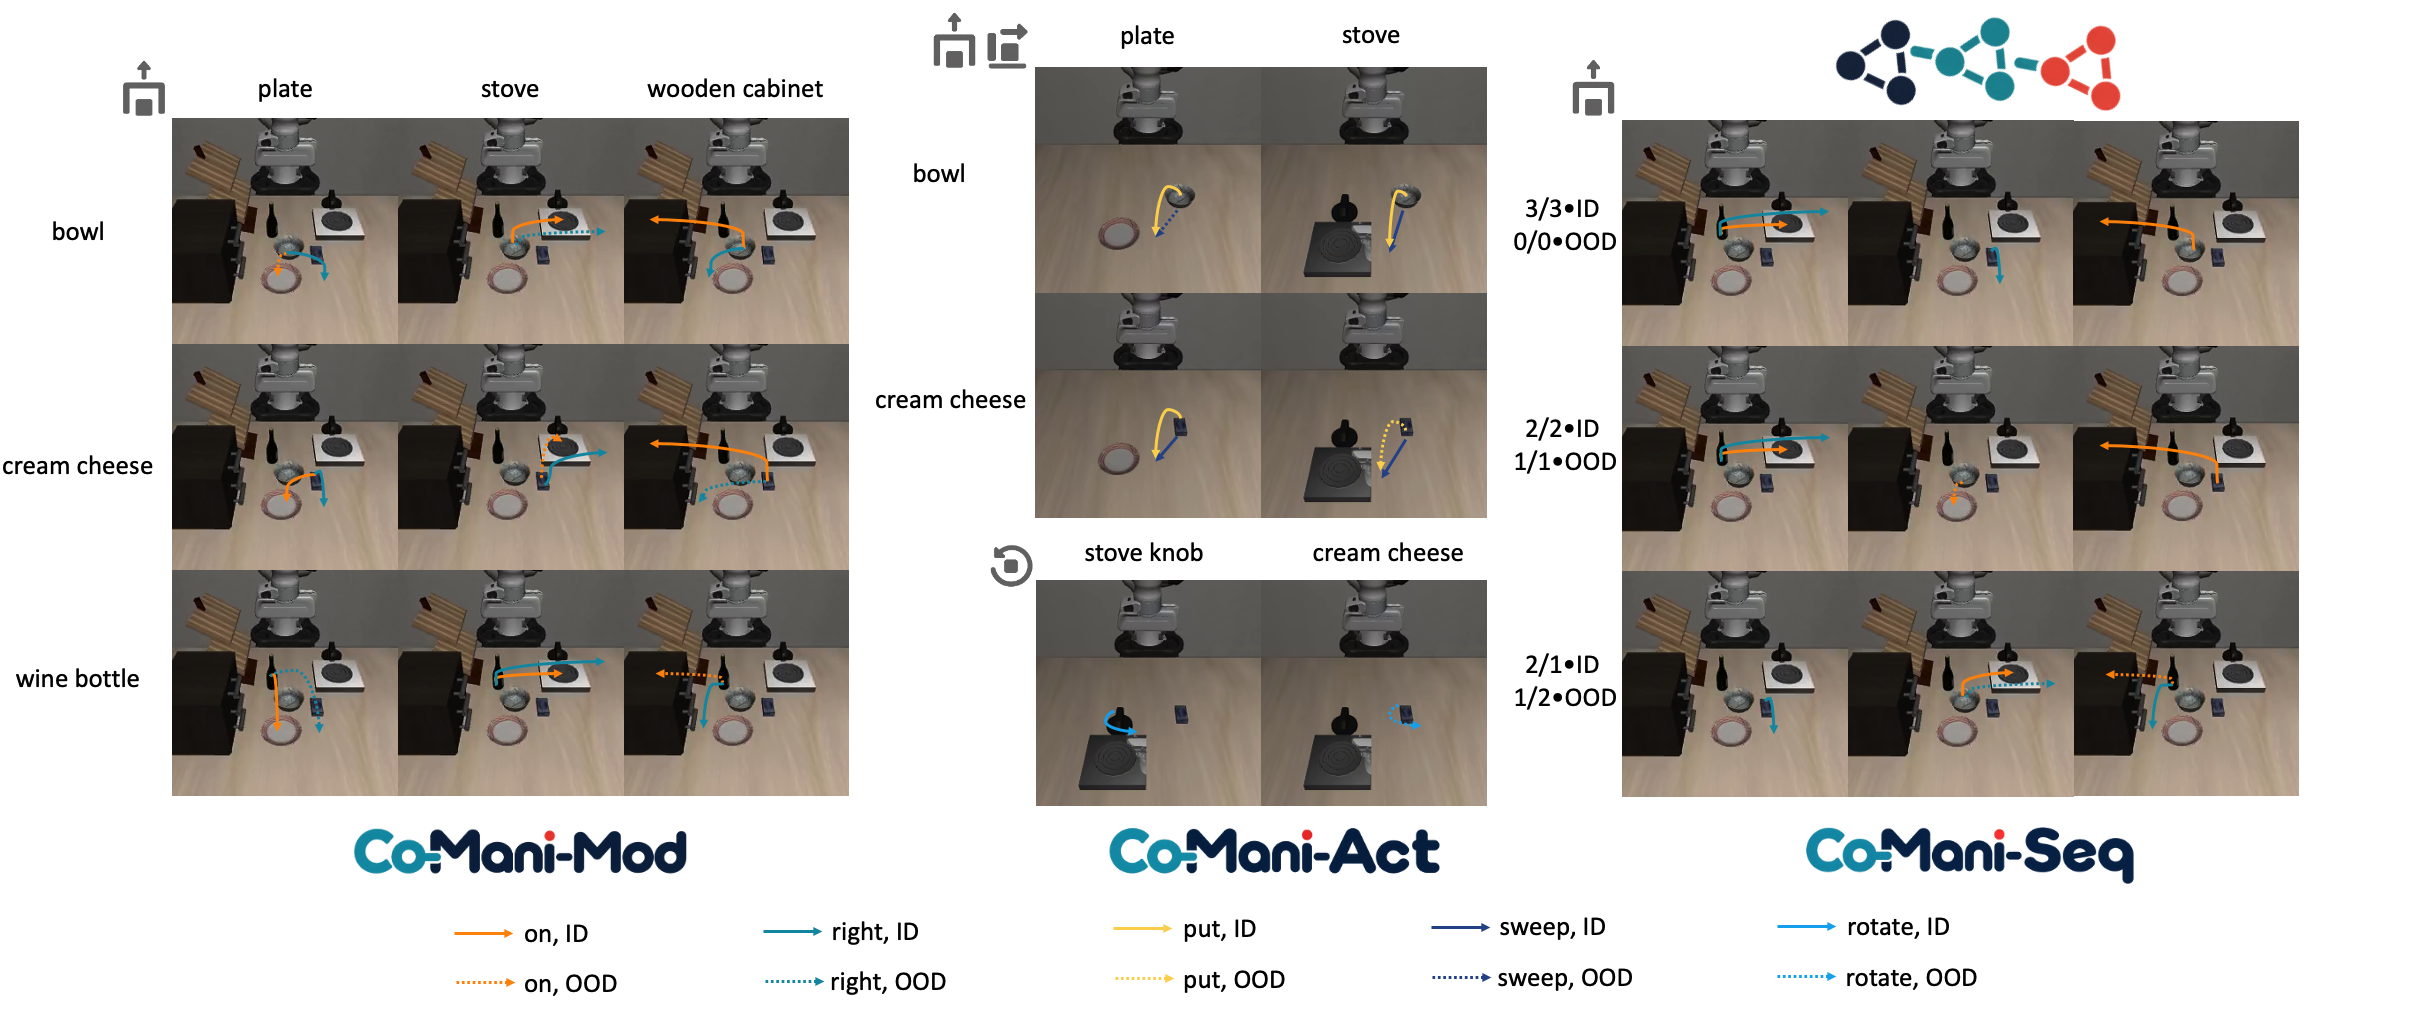
\includegraphics[width=\textwidth]{fig/benchmark.png}
    \caption{CoMani task construction and splits.
    Left: CoMani-Mod varies modifiers with a fixed put action.
    Center: CoMani-Act varies action types with a fixed right modifier.
    Right: CoMani-Seq composes atomic tasks from CoMani-Mod into six three-step sequences, shown in three rows with execution proceeding from left to right.}
    \label{fig:benchmark}
\end{figure*}

% Figure corrections pending: in the CoMani-Mod legend, dotted yellow means
% on/OOD and solid blue means right/ID.

\textbf{CoMani-Mod.} With pick-and-place (\emph{put}) fixed, this suite combines 3 objects, 3 targets, and 2 modifiers (\emph{on}/\emph{right of}) into 18 tasks: 12 in-distribution (ID) and 6 out-of-distribution (OOD).
Each OOD object--target pair appears in the ID split with the opposite modifier, isolating generalization to unseen combinations of familiar factors.
The ID/OOD comparison therefore tests whether a policy can apply the instructed relation to a familiar object--target pair beyond its demonstrated placement.

% Internal suite: 0902. Code ID-split IDs: 1,2,3,5,6,8,9,10,12,13,16,17.
% OOD IDs: 0,4,7,11,14,15. Held-out on: bowl/plate, cheese/stove,
% bottle/cabinet. Held-out right: bowl/stove, cheese/cabinet, bottle/plate.

\textbf{CoMani-Act.} With \emph{right} fixed, this suite varies \emph{put}, \emph{sweep}, and \emph{rotate} across 10 tasks: 7 ID and 3 OOD.
For put/sweep, each OOD object--target pair appears in the ID split with the other action; for rotation, the ID task uses the stove knob and the OOD task uses cream cheese.
These tests examine whether a policy can reuse an action with familiar entities in a new combination and transfer rotation across different manipulated entities.
Put/sweep pairs share initial states and final-position goals, so success measures goal attainment rather than interaction mode.

% Internal suite: 0904. Code ID-split IDs: 0,1,2,5,7,8,9. Code OOD-split IDs: 3,4,6.
% Rotation details: dataset term "right" means counterclockwise about world +Z
% viewed from above. Knob: joint position >= 0.5 rad. Cheese: reset-relative
% signed rotation >= 0.5 rad, with tilt <= 15 degrees.

\textbf{CoMani-Seq.} This suite tests whether policies learned from CoMani-Mod atomic demonstrations can execute 3-step instructions without sequence-level demonstrations.
It contains 6 sequences organized into 3 fixed-order pairs, each varying one modifier between \emph{on} and \emph{right of}, without permuting subtasks.
The 3 pairs contain 3 ID, 2 ID + 1 OOD, and 2/1 ID + 1/2 OOD atomic tasks, respectively (Fig.~\ref{fig:benchmark}, right).
The all-ID pair tests composition and transitions among familiar skills; the remaining pairs test whether execution also generalizes to held-out atomic combinations, with the last pair increasing the OOD count from 1 to 2 through a single modifier change.

% Internal suite: libero_custom_0906. Evaluation order: 0,1,2,3,4,5.
% Figure pair order: tasks 2/3 (3 ID), 0/1 (2 ID + 1 OOD), 4/5 (mixed).
% TODO: Specify shared-scene initialization, ordered subtask completion checks,
% whether earlier goals must remain satisfied, and the sequence time budget.
\begin{table*}[t]
\centering
\caption{CoMani task lists and ID/OOD splits.
In (c), ID/OOD gives atomic task counts; atomic IDs refer to (a), with OOD IDs underlined.}
% IMPORTANT: Paper IDs differ from code/evaluation IDs.
% Use expr/task_id_mapping.json when importing results; never match numeric IDs directly.
\label{tab:comani_tasks}
\footnotesize
\setlength{\tabcolsep}{2pt}
\renewcommand{\arraystretch}{1.08}
\begin{minipage}[t]{0.49\textwidth}
\centering
\textbf{(a) CoMani-Mod}\par\smallskip
% Match the height of the stacked Act and Seq tables on the right.
\renewcommand{\arraystretch}{1.532}
\begin{tabular*}{\linewidth}{@{\extracolsep{\fill}}r|p{6.35cm}|l}
\noalign{\hrule height 1pt}
ID & Task instruction & Split \\
\hline
0 & Put the bowl on the stove. & ID \\
1 & Put the bowl on the wooden cabinet. & ID \\
2 & Put the bowl to the right of the plate. & ID \\
3 & Put the bowl to the right of the wooden cabinet. & ID \\
4 & Put the cream cheese on the plate. & ID \\
5 & Put the cream cheese on the wooden cabinet. & ID \\
6 & Put the cream cheese to the right of the plate. & ID \\
7 & Put the cream cheese to the right of the stove. & ID \\
8 & Put the wine bottle on the plate. & ID \\
9 & Put the wine bottle on the stove. & ID \\
10 & Put the wine bottle to the right of the stove. & ID \\
11 & Put the wine bottle to the right of the wooden cabinet. & ID \\
\hline
12 & Put the bowl on the plate. & OOD \\
13 & Put the bowl to the right of the stove. & OOD \\
14 & Put the cream cheese on the stove. & OOD \\
15 & Put the cream cheese to the right of the wooden cabinet. & OOD \\
16 & Put the wine bottle on the wooden cabinet. & OOD \\
17 & Put the wine bottle to the right of the plate. & OOD \\
\noalign{\hrule height 1pt}
\end{tabular*}
\end{minipage}\hfill
\begin{minipage}[t]{0.49\textwidth}
\centering
\textbf{(b) CoMani-Act}\par\smallskip
\begin{tabular*}{\linewidth}{@{\extracolsep{\fill}}r|p{6.35cm}|l}
\noalign{\hrule height 1pt}
ID & Task instruction & Split \\
\hline
0 & Put the bowl to the right of the plate. & ID \\
1 & Put the bowl to the right of the stove. & ID \\
2 & Put the cream cheese to the right of the plate. & ID \\
3 & Rotate the stove knob right. & ID \\
4 & Sweep the bowl to the right of the stove. & ID \\
5 & Sweep the cream cheese to the right of the plate. & ID \\
6 & Sweep the cream cheese to the right of the stove. & ID \\
\hline
7 & Put the cream cheese to the right of the stove. & OOD \\
8 & Rotate the cream cheese right. & OOD \\
9 & Sweep the bowl to the right of the plate. & OOD \\
\noalign{\hrule height 1pt}
\end{tabular*}
\par\smallskip
\centering
\textbf{(c) CoMani-Seq}\par\smallskip
\begin{tabular*}{\linewidth}{@{\extracolsep{\fill}}r|l|p{4.7cm}|l}
\noalign{\hrule height 1pt}
ID & ID/OOD & Sequence & Atomic IDs \\
\hline
0 & 3/0 & Wine bottle on stove $\to$ cream cheese right of plate $\to$ bowl on wooden cabinet & $9\to6\to1$ \\
1 & 3/0 & Wine bottle right of stove $\to$ cream cheese right of plate $\to$ bowl on wooden cabinet & $10\to6\to1$ \\
\hline
2 & 2/1 & Wine bottle on stove $\to$ bowl on plate $\to$ cream cheese on wooden cabinet & $9\to\underline{12}\to5$ \\
3 & 2/1 & Wine bottle right of stove $\to$ bowl on plate $\to$ cream cheese on wooden cabinet & $10\to\underline{12}\to5$ \\
\hline
4 & 2/1 & Cream cheese right of plate $\to$ bowl on stove $\to$ wine bottle on wooden cabinet & $6\to0\to\underline{16}$ \\
5 & 1/2 & Cream cheese right of plate $\to$ bowl right of stove $\to$ wine bottle on wooden cabinet & $6\to\underline{13}\to\underline{16}$ \\
\noalign{\hrule height 1pt}
\end{tabular*}
\end{minipage}
\end{table*}
